\documentclass{beamer}

\usepackage{beamerthemesplit}
\usepackage{amsmath}
\usepackage{amsfonts}
\usepackage{amssymb}
\usepackage{qtree}
\usepackage{cancel}
\usepackage{tkz-graph}
%\usepackage[pdftex]{graphicx}

\mode<presentation>
{
  \usetheme{Warsaw}
  % or ...

  %\setbeamercovered{transparent}
  % or whatever (possibly just delete it)
}


\usepackage[english]{babel}
% or whatever

\usepackage[latin1]{inputenc}
% or whatever

\usepackage{times}
\usepackage[T1]{fontenc}


%%%%%%%%% NEW COMMANDS %%%%%%%%%
\newcommand{\score}{{\it score}}
\newcommand{\fitness}{{\it fitness}}
\newcommand{\sizepenalty}{{\it sizePenalty}}
\newcommand{\pset}[1]{\Theta_i(#1)}
\newcommand{\argmax}[1]{\underset{#1}{\operatorname{argmax}}\ }
\newcommand{\argmin}[1]{\underset{#1}{\operatorname{argmin}}\ }
\newcommand{\stos}{f_i}
\newcommand{\stof}{g_i}


\title{Imitation \& Reinforcement Learning}

\subtitle{in Virtually Embodied Agents Using Program Evolution}

\author{Nil Geisweiller}

\institute[Xiamen University] % (optional, but mostly needed)
{
  Novamente LLC
}

\date[Xiamen University AGI Summer School 2009] % (optional, should be abbreviation of conference name)
{Xiamen University\\ AGI Summer School 2009}


\AtBeginSection[]
{
  \begin{frame}<beamer>{Outline}
    \tableofcontents[currentsection,currentsection]
  \end{frame}
}

\AtBeginSubsection[]
{
  \begin{frame}<beamer>{Outline}
    \tableofcontents[currentsection,currentsubsection]
  \end{frame}
}

%\newcommand{\AND}{\textit{AND}}
%\newcommand{\OR}{\textit{OR}}
%\newcommand{\NOT}{\textit{NOT}}
\newcommand{\AND}{\land}
\newcommand{\OR}{\lor}
\newcommand{\NOT}{\lnot}


\begin{document}

\frame
{
  \maketitle
}
\section[Outline]{}
\frame{\tableofcontents}

\section{Introduction}

\frame
{
  \frametitle{Introduction}

  \begin{beamerboxesrounded}{Imitation \& Reinforcement Learning}
    A way to communicate
      \alert{procedural knowledge without programming}
      or sophisticated \alert{NLP}
  \end{beamerboxesrounded}

  \begin{columns}

    \column{1in}

    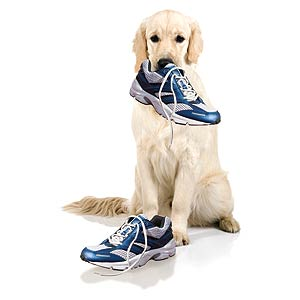
\includegraphics[scale=0.3]{dog_shoes.jpg}
 
    \column{2in}

    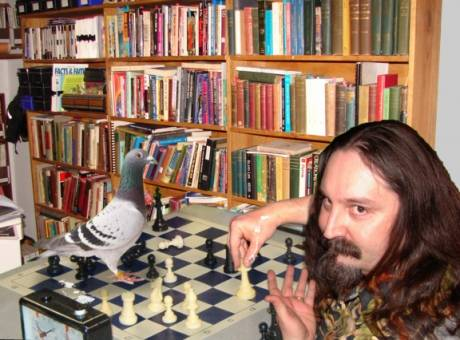
\includegraphics[scale=0.3]{pigeon-chess.jpg}
    
  \end{columns}
}

\frame
{
  \frametitle{\alert{Imitation Reinforcement Loop} in Embodiment}

  \begin{center}
    \only<1>{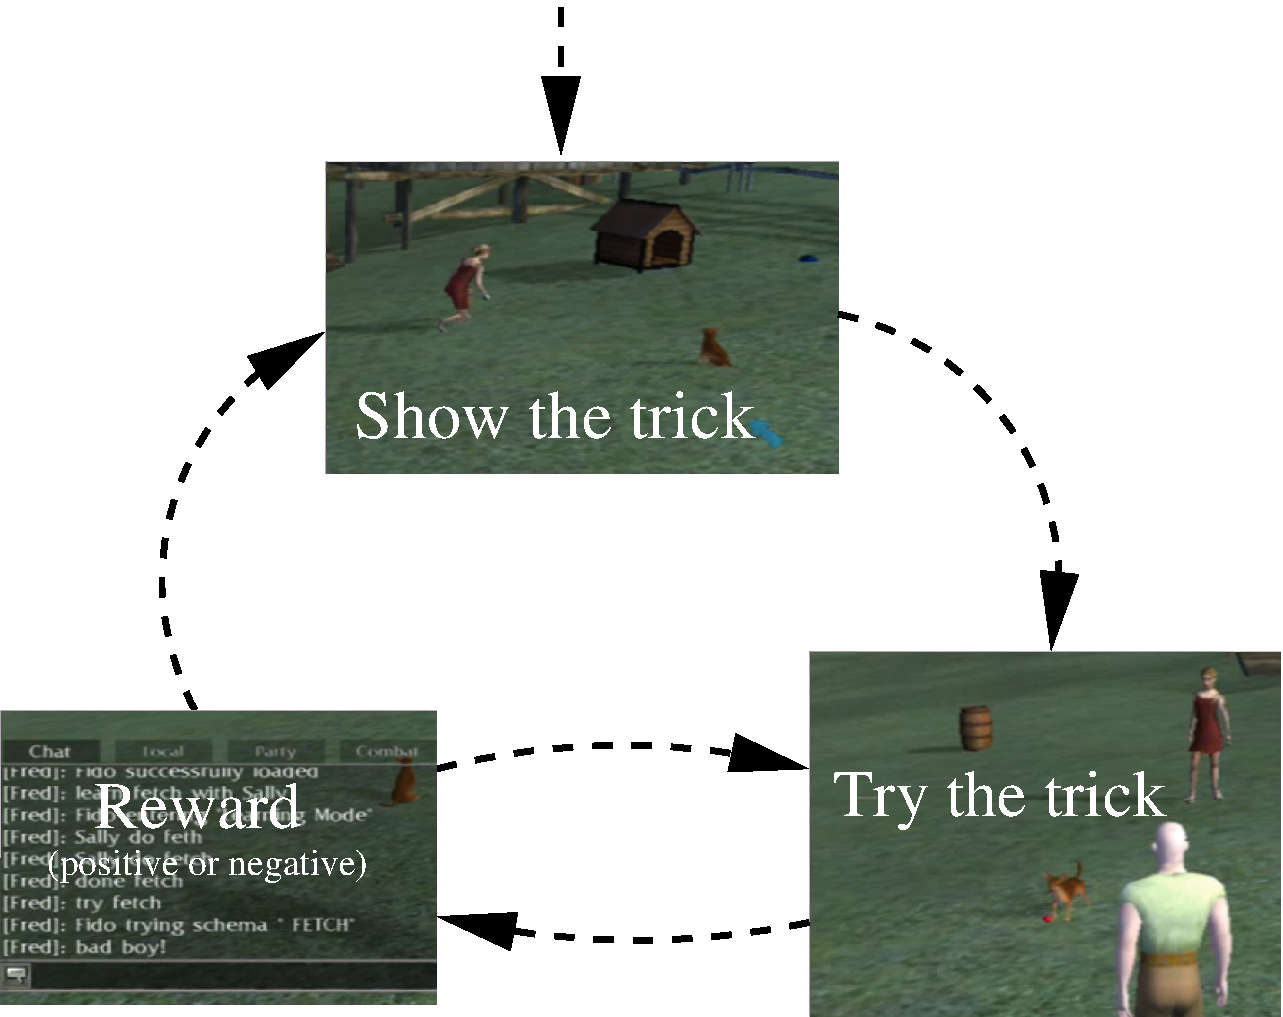
\includegraphics[scale=0.3]{imitation_cycle.pdf}}
    \only<2>{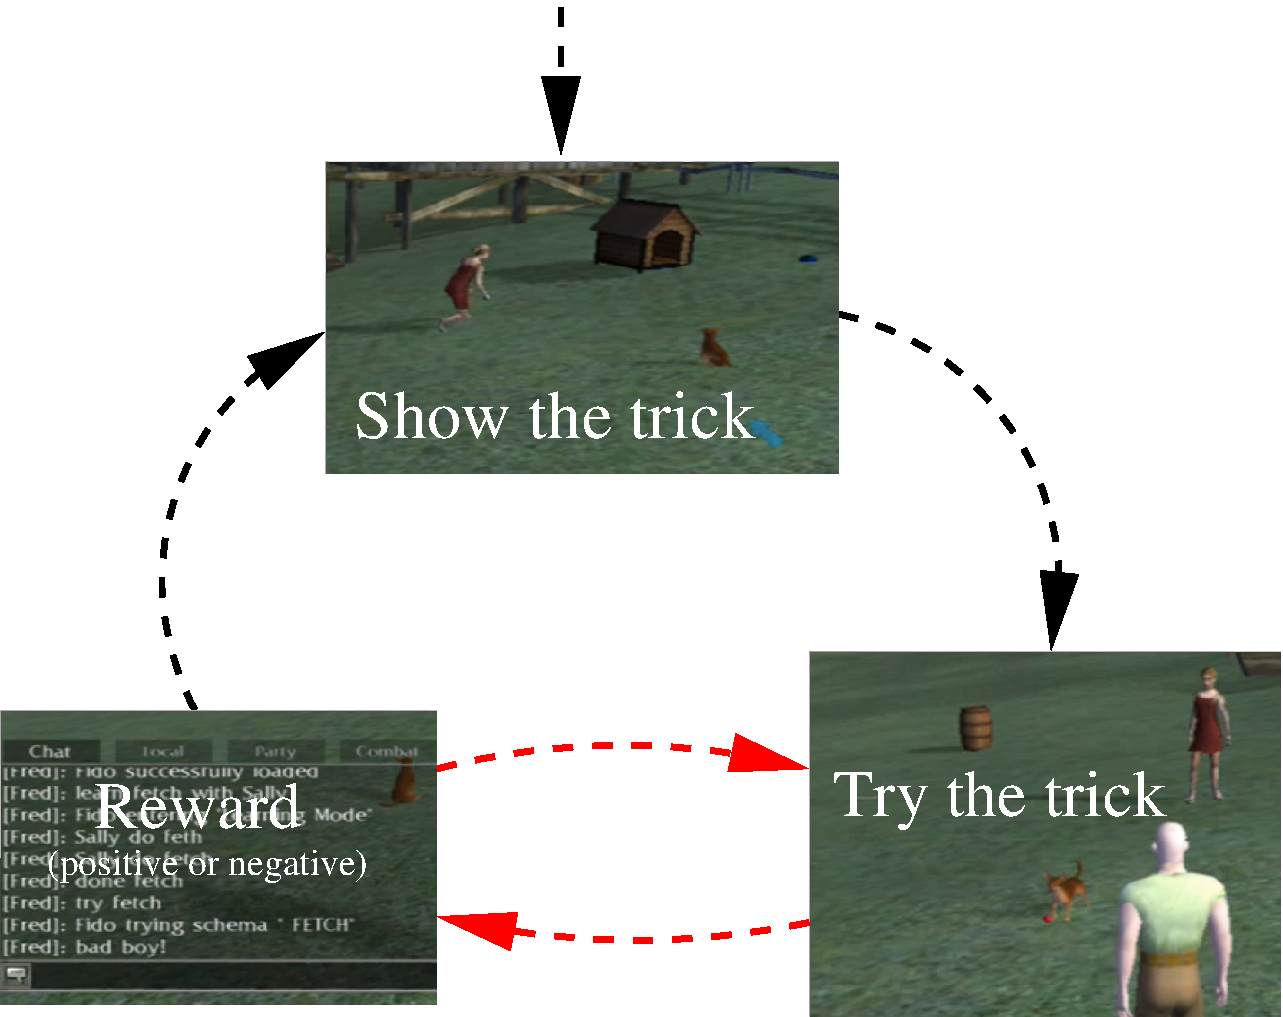
\includegraphics[scale=0.3]{imitation_cycle_red.pdf}}
  \end{center}
  \begin{enumerate}
  \item<+-> How to find \alert{rapidely a trick that fits}?
  \item<+-> How to \alert{take reward into account} to \alert{converge faster}?
  \end{enumerate}

}

\section{Searching the Space of Trick Candidates}

\subsection{Overview}

\frame
{
  \frametitle{Searching the Space of Trick Candidates: Recall}

  \begin{enumerate}
  \item<+-> Operational Agent Controller (OPC) \alert{provides}
    the \alert{episodic memory
    of the learning session} to HillClimbing (or MOSES)
  \item<+-> Which \alert{searches
    the program space} to find one that fits (\alert{mimics avatar's behavior})
  \end{enumerate}

  \begin{columns}
    \column{1.5in}
    \visible<1->{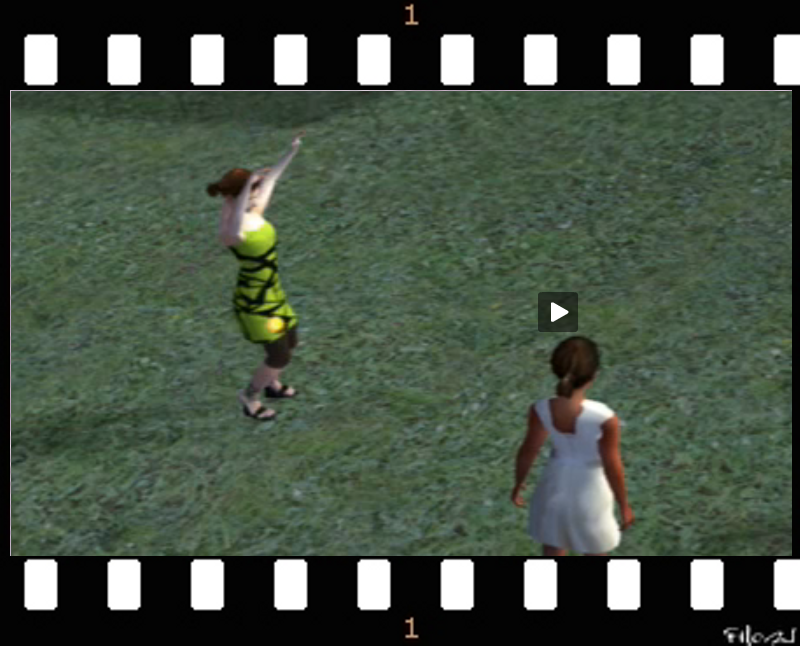
\includegraphics[scale=0.17]{movie_jill.png}}
    
    \column{2in}
    \visible<2->{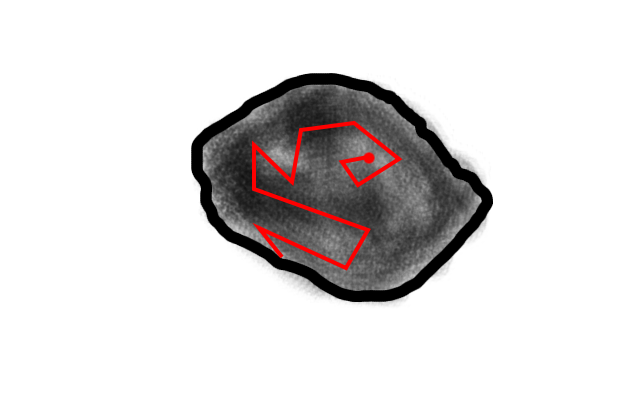
\includegraphics[scale=0.3]{program_space.png}}
  \end{columns}

}

\frame
{
  \frametitle{The pet \alert{replaies mentally} the scene,
    but \alert{substitues the avatar to imitate by itself}}
  \begin{columns}
    \column{1.9in}
    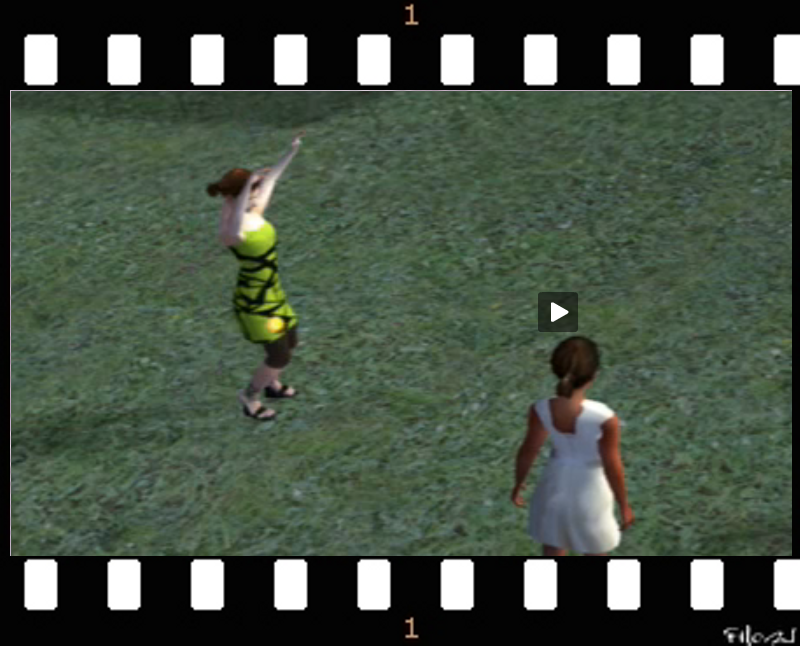
\includegraphics[scale=0.17]{movie_jill.png}
    \column{0.1in}
    $\Rightarrow$
    \column{2in}
    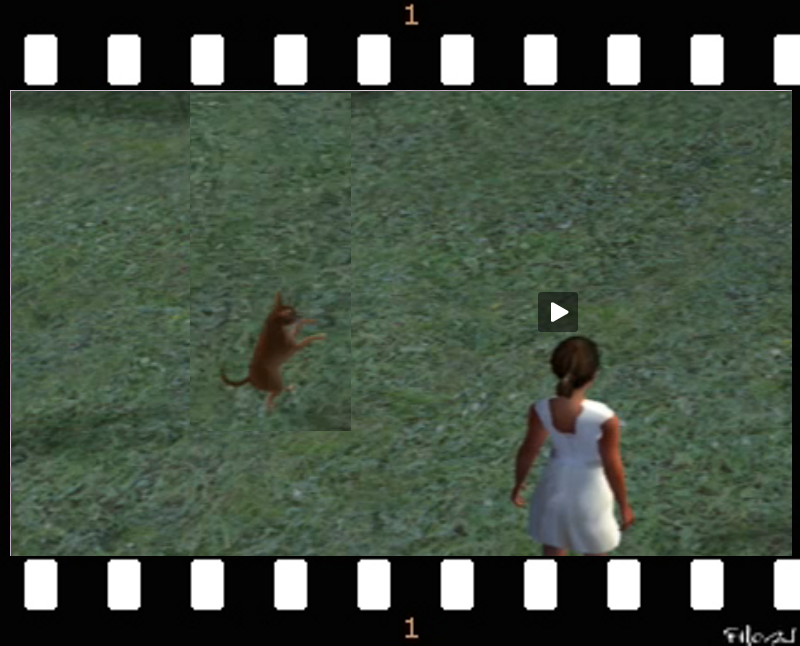
\includegraphics[scale=0.17]{movie_fido.png}
  \end{columns}

  \begin{beamerboxesrounded}{Fitness Function}
    Measure how the program
    \alert{candidate's behavior fits the avatar's}
    (compare their sequence of actions)
  \end{beamerboxesrounded}
}

\frame
{
  \frametitle{\alert{Operators involved} to build program candidates}

  \begin{columns}
    \column{1.7in}
    {\footnotesize
    {\tt
      \begin{itemize}
      \item \alert<2>{sequential\_and}
      \item \alert<2>{action\_boolean\_if}
      \item action\_action\_if
      \item action\_while
      \item \alert<2>{boolean\_while}
      \item action\_not
      \item \alert<2>{logical\_not}
      \item random\_object
      \item nearest\_object
      \end{itemize}
    }
    }
    \column{0.1in}
    +
    \column{1.8in}
    \begin{itemize}
    \item Potential perceptions, {\small {\tt near(obj\_1 obj\_2)}},
      {\small {\tt is\_moving(obj\_3)}}, etc.
    \item Potential actions, {\small {\tt grab(obj\_1)}},
      {\small {\tt goto\_obj(avatar\_2)}}, etc.
    \end{itemize}
  \end{columns}
}

\frame[containsverbatim]
{
  \frametitle{Example of Tricks in Combo}

\begin{enumerate}
\item Fetch a random object
{\footnotesize
\begin{verbatim}
and_seq(goto_obj(random_object)
        grab(nearest_object)
        goto_obj(owner)
        drop)
\end{verbatim}
}
\item kicks 3 times,
  from the left leg if stick is near ball and from the right leg otherwise
{\footnotesize
\begin{verbatim}
action_if(near(stick ball)
          and_seq(kickLeft kickLeft kickLeft)
          and_seq(kickRight kickRight kickRight))
\end{verbatim}
}
\item Dance on cue until the owner says ``stop dancing''
{\footnotesize
\begin{verbatim}
boolean_while(not(has_said(owner "stop dancing"))
              action_if(is_last_action(owner "kickL")
                        tap_dance
                        lean_rock_dance))
\end{verbatim}
}
\end{enumerate}

}

\frame
{
  \frametitle{HillClimbing Search Algo}

  \begin{center}
  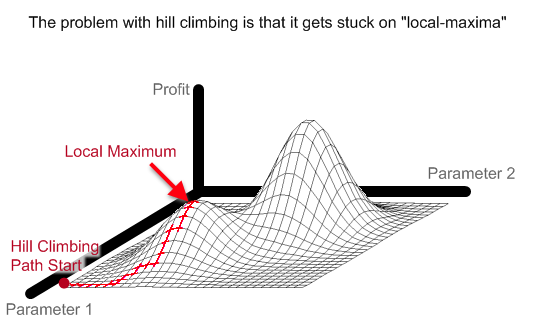
\includegraphics[scale=0.3]{HillClimbingLocalMax.png}
  \end{center}

  HillClimbing + restart on the best non yet restarted candidate
}

\subsection{Accelerating Search}

\frame
{
  \frametitle{Accelerating HillClimbing Search}

  \begin{enumerate}
  \item<+-> Reduction in normal form to avoid over representation
  \item<+-> Filtering Perceptions, entropy threshold
  \item<+-> Building-blocks of action sequences
  \item<+-> Setting carefully Occam's razor function
  \end{enumerate}
}

\frame
{
  \frametitle{Filtering Perception, Entropy Threshold}
  \[c<-\sum_{i={1,2}} p_i \times {\it log}_2(p_i)\]
  Example, entropy of {\tt near(chair1 chair2)} is null
  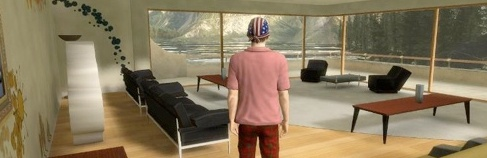
\includegraphics[scale=0.35]{office_crop.jpg}
}

\frame[containsverbatim]
{
  \frametitle{Building-blocks of action sequences}

Example with fetch:

\begin{enumerate}
\item
{\footnotesize
\begin{verbatim}
and_seq(goto_obj(random_object)
        grab(nearest_object)
        goto_obj(owner)
        drop)
\end{verbatim}
}
\item
{\footnotesize
\begin{verbatim}
and_seq(goto_obj(nearest_object)
        grab(nearest_object)
        goto_obj(owner)
        drop)
\end{verbatim}
}
\item
{\footnotesize
\begin{verbatim}
and_seq(goto_obj(ball)
        grab(ball)
        goto_obj(owner)
        drop)
\end{verbatim}
}
\item
$\ldots$
\end{enumerate}

It may be faster to start from the sequence itself rather than an empty program.
}

\frame
{
  \frametitle{Setting carefully Occam's razor function}
  \begin{itemize}
  \item<+-> Problem,
    when the sequence is \alert{too long it easily generates over-complicated
    candidates}
  \item<+-> Solution, strong \alert{bias toward simple candidates}
    first even if
    they fit less.
    
  \item<+-> Automatically tuning $\sizepenalty_{a,b}$
    \alert{based on the past learning experiences}
    \[\sizepenalty_{a,b}(p)
    = exp(-a \times log(b \times |A|+exp(1)) \times |p|)\]
    

  \end{itemize}
}

% \frame
% {
%   \frametitle{Setting carefully Occam's razor function}
%   TODO: show screenshot of python code and logging trace

%   And conclude with printing in atom table the trace and using the entire
%   OpenCog system to improve the algo.

%   So opencog as a tool to improve (interactively or not) itself
% }

\frame
{
  \frametitle{Some benchmarks}

{\tiny

\begin{columns}

\column{2in}

\begin{table}
\center
\begin{tabular}{|r|r|r|r||c|}
\hline
Reduct & ActSeq & Entropy & Occam & Setting \\
\hline
On & Off & 0.1   & 0.03 & {\it conf}$_1$ \\
Off & Off & 0.1  & 0.03 & {\it conf}$_3$ \\
On & Off & 0     & 0.03 & {\it conf}$_4$ \\
On & Off & 0.1   & 0.3 & {\it conf}$_7$ \\ 
On & On & 0.1  & 0.03 & {\it conf}$_9$ \\
On & On & 0.1 & 0.025 & {\it conf}$_{10}$ \\
\hline
\end{tabular}
\caption{Settings for each learning experiment}
\label{table:settings}
\end{table}

%ENTROPY TIME = 0.32

\column{1.5in}

\begin{table}
\center
\begin{tabular}{|c||r|r|r|r|}
\hline
Setting & Eval & Time \\
\hline
{\it conf}$_1$  & 653   & 5s18 \\
{\it conf}$_3$  & 1073  & 8s42 \\
{\it conf}$_4$  & 28287 & 4mn7s \\
{\it conf}$_7$  & 3121  & 23s42 \\
{\it conf}$_9$  & 89 & 410ms \\
{\it conf}$_{10}$  & 33 & 161ms \\
\hline
\end{tabular}
\caption{fetch\_ball}
\label{table:fetch}
\end{table}

\end{columns}

\begin{columns}

\column{1.5in}

%ENTROPY TIME = 0.05

\begin{table}
\center
\begin{tabular}{|c||r|r|r|r|}
\hline
Setting & Eval & Time \\
\hline
{\it conf}$_1$  & 2783  & 21s47 \\
{\it conf}$_3$  & 15069 & 2mn15s \\
{\it conf}$_4$  & $\infty$ & $\infty$ \\
{\it conf}$_7$  & $>$200K  & $>$1h \\
{\it conf}$_9$  & 107 & 146ms \\
{\it conf}$_{10}$  & 101 & 164ms \\
\hline
\end{tabular}
\caption{triple\_kick}
\label{table:triplekick}
\end{table}

%\subsubsection{Double\_dance}

\column{1.5in}

%ENTROPY TIME = 3.15

\begin{table}
\center
\begin{tabular}{|c||r|r|r|r|}
\hline
Setting & Eval & Time \\
\hline
{\it conf}$_1$  & 113  & 4s \\
{\it conf}$_3$  & 150  & 6s20ms \\
{\it conf}$_4$  & $>$60K & $>$1h \\ 
{\it conf}$_7$  & 113  & 4s \\
{\it conf}$_9$  & 138 & 4s191ms \\
{\it conf}$_{10}$  & 219K & 56mn3s \\
\hline
\end{tabular}
\caption{double\_dance}
\label{table:doubledance}
\end{table}

\end{columns}

}

}

\frame[containsverbatim]
{
  \frametitle{Example of Tricks in Combo}

\begin{enumerate}
\item fetch\_ball
{\footnotesize
\begin{verbatim}
and_seq(goto_obj(ball)
        grab(ball)
        goto_obj(owner)
        drop)
\end{verbatim}
}
\item triple\_kick
{\footnotesize
\begin{verbatim}
action_if(near(stick ball)
          and_seq(kickLeft kickLeft kickLeft)
          and_seq(kickRight kickRight kickRight))
\end{verbatim}
}
\item double\_dance
{\footnotesize
\begin{verbatim}
boolean_while(not(has_said(owner "stop dancing"))
              action_if(is_last_action(owner "kickL")
                        tap_dance
                        lean_rock_dance))
\end{verbatim}
}
\end{enumerate}
}
\section{Taking Reward into Account}

\frame
{
  \frametitle{\alert{Taking Reward into Account} to Converge Faster
    (Not implemented yet)}

  \begin{center}
    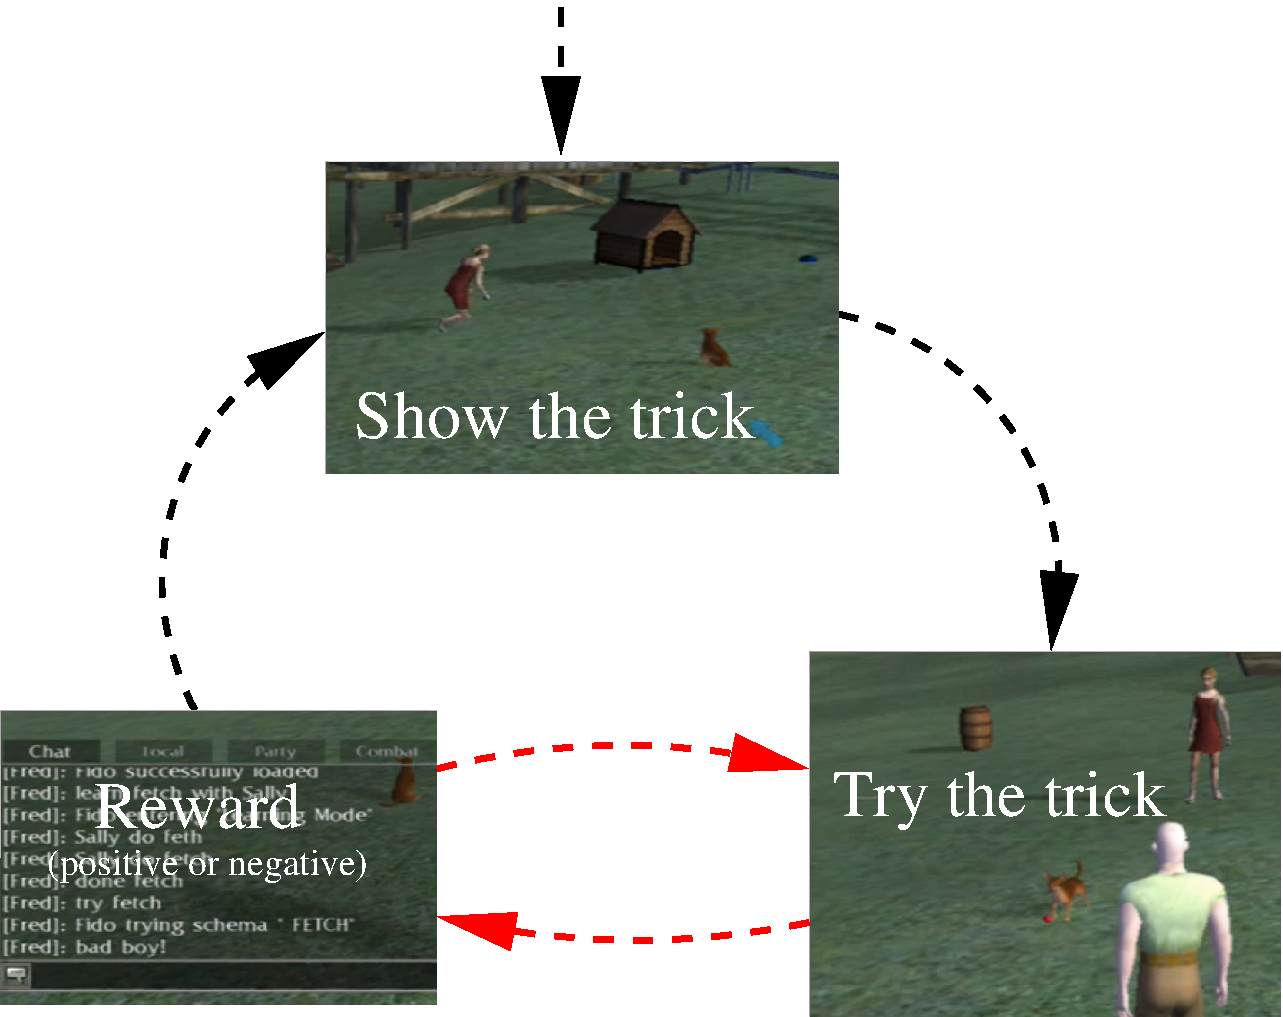
\includegraphics[scale=0.3]{imitation_cycle_red.pdf}
  \end{center}
}

\frame
{
  \frametitle{\alert{Taking Reward into Account} to Converge Faster
    (Not implemented yet)}

  \begin{beamerboxesrounded}{Main idea}
    Use the pet's trial as new \alert{exemplar weighted by owner's reward}
  \end{beamerboxesrounded}

  \begin{columns}
    \column{0.5in}
    Fitness
    \column{0.1in}
    $\leftarrow$
    \column{2.6in}
    \begin{itemize}
    \item new episodes taken into account
    \item candidate to be compared
      to be \alert{similar to a good trials} or 
      \alert{dissimilar to a bad trials}.
    \end{itemize}
  \end{columns}
}
\section{Conclusion}

\frame
{
  \frametitle{Conclusion}

  Pretty fast on simple tricks but...\\[2ex]

  What remains to be done:
  \begin{itemize}
  \item<+-> \alert{Improve Mental image of the scene} to be more accurate
    (action consequence, collisions)
  \item<+-> Take into account that \alert{pet is not human (co-evolution)}
  \item<+-> Implement owner reward feedback for faster convergence
  \item<+-> Improving Filters by using \alert{Attention Allocation}
  \item<+-> Extend SizePenalty Bias to all parameters of the search algo
    (distribution priors, etc), \alert{Transfer Learning}
  \end{itemize}
}

\end{document}